\documentclass[../EngineeringJournal_CDavis.tex]{subfiles}

\begin{document}

%%%%%%%%%%%%%%%%%%%%%%%%%%%%%%%%%%%%%%%%%%%%%%%%%%%%%
%%%%%%%%%%%%%%%%%%%%%%%%%%%%%%%%%%%%%%%%%%%%%%%%%%%%%

\chapter[Troubleshooting Static Routes]{Troubleshooting \linebreak[1] Static Routes \hspace*{\fill}{Feb 4, 2020}}
\noindent\textbf{{Packet Tracer Lab 4} \hspace*{\fill}{\textbf{CIT 167}}}\linebreak[1]
{{Spring 2020} \hspace*{\fill}{Chaz Davis}}                             
%===================================
%===================================

\hspace{0.2cm}
\begin{tcolorbox}[width=6.3in]
\scriptsize 
- Important Commands for the Lab
  \begin{itemize}
    \item{show ip route [ip-address]} to display the current state of the routing table
      \subitem{command can be used in EXEC or privileged EXEC mode}
    \item{no ip route} To remove static routes, use this command in global configuration
      \subitem{ {\scriptsize{\verb$no ip route prefix mask <ip address | interface-type interface-number> [permanent]$}\normalsize} } 
    \item{ip route} To establish static routes, use this command in global configuration 
      \subitem{ {\scriptsize{\verb$ip route prefix mask <ip address | interface-type interface-number> [permanent]$}\normalsize} } 
        \subitem{ {\scriptsize{\verb$ip route 192.168.3.0 255.255.255.0 192.168.2.2$}\normalsize} } 
  \end{itemize}
\end{tcolorbox}
\hspace{0.2cm}
\normalsize  

\newpage

%===================================
\mysection{\textbf{Part 1: Locate The Problem}}
Based on the output of the commands I've run, from PC1 and from R1 and R2 and R3. 
\\It appears that R2 is incorrectly configured and it has R1 as the wrong ip adresses
in its routing table. See Fig.
\\It also appears that R3 is incorrectly configured and has no route for pc1 in its
tables.


\begin{figure}[!hbt]\centering
\subfloat[R2 misconfiguration of static
Route]{\label{msconfig4R2}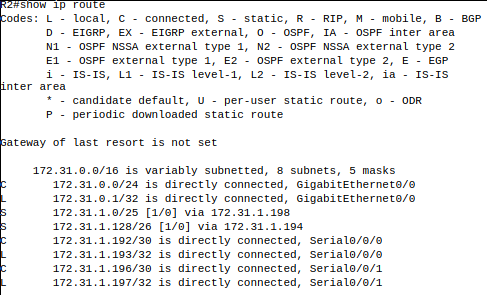
\includegraphics[width=.55\linewidth]{Figures/2020-02-09-155109_487x295_scrot.png}}\par
\caption{Network Misconfigured: \\R2 - not set up for R1}
\label{misconfig4}
\end{figure}




%===================================
\mysection{\textbf{Part 2: Determine the solution}}
I believe the solution is going to be statically configuring the routes for router 2 and 3, making sure that all are connected.

%===================================
\mysection{\textbf{Part 3: Implement the solution}}

I went to R2 first, and configured the network settings. First, by removing the
incorrect routing tables by running the 
\\commands {\scriptsize{\verb$no ip route 172.31.1.0 255.255.255.128 172.31.1.198$}\normalsize} and {\scriptsize{\verb$no ip route 172.31.1.128 255.255.255.192 172.31.1.194$}\normalsize}  Then, I repopulated the table by running the 
\\commands {\scriptsize{\verb$ip route 172.31.1.0 255.255.255.128 172.31.1.194$}\normalsize} and {\scriptsize{\verb$ip route 172.31.1.128 255.255.255.192 172.31.1.198$}\normalsize}. 
\\I then went to R3 and cofigured it for PC1 by running {\scriptsize{\verb$ip route 172.31.1.0 255.255.255.128 serial 0/0/1$}\normalsize} 


%===================================
\mysection{\textbf{Part 4: Verify that the issue is resolved}}
Finally I verified that the network is now working properly. Table on
Pg.~\pageref{success4}
\\As you can see in FIg.~\ref{success4}\subref{success4ping1} I was successfully able to ping the server from PC1. 
\\I then opened the web browser on PC1 Fig.~\ref{success4}\subref{success4web1} and PC2
Fig.~\ref{success4}\subref{success4web2} and entered the servers
address and got the congratulations message.


\begin{figure}[!hbt]\centering
\subfloat[Successful Ping of the server from
PC1]{\label{success4ping1}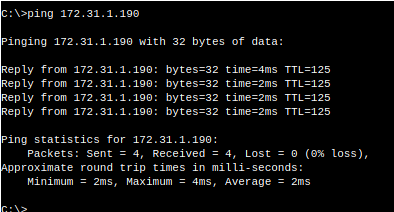
\includegraphics[width=.45\linewidth]{Figures/2020-02-09-161308_394x212_scrot.png}}\par
\subfloat[Successful Webpage Login
PC1]{\label{success4web1}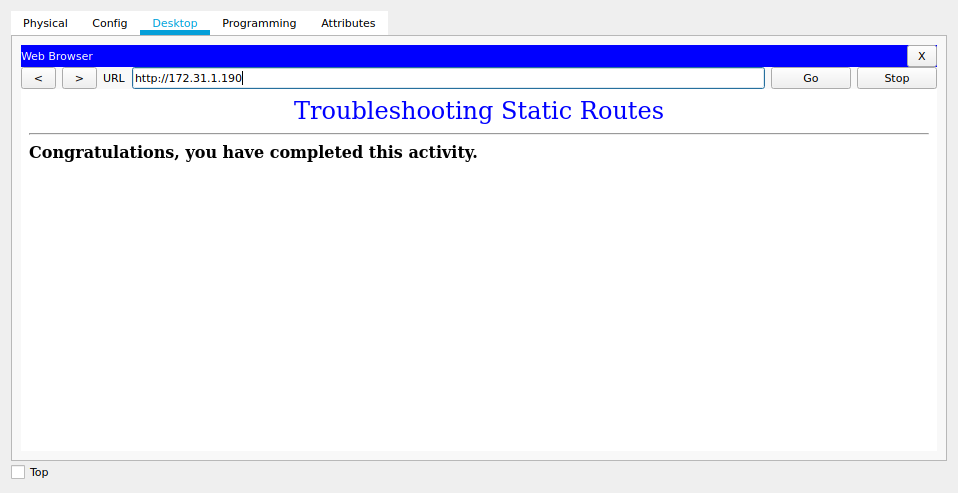
\includegraphics[width=.45\linewidth]{Figures/2020-02-09-161510_958x493_scrot.png}}\hfill
\subfloat[Successful Webpage Login from
PC2]{\label{success4web2}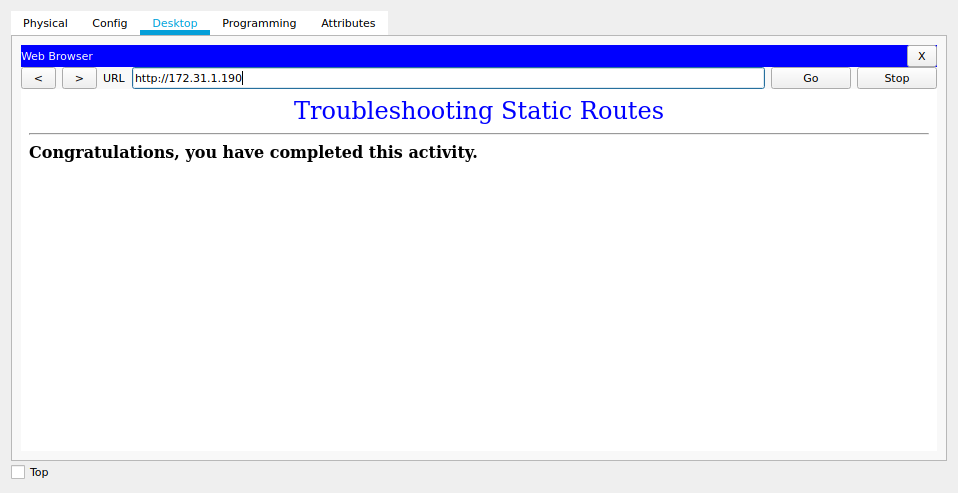
\includegraphics[width=.45\linewidth]{Figures/2020-02-09-161602_958x493_scrot.png}}\par
\caption{Successful Verification}
\label{success4}
\end{figure}




%===================================

\end{document}
